%======================================================================
\subsection{BW-UIX-08 --- Plan and build: the Fusion-like studio look (25 Oct 2026)}\label{sec:uix08-plan}
%======================================================================

\eref{UIX-08} answers the 25 Oct UAT, item \#6: ``better visual rendering with textures''. Asked which look, you chose
\textbf{Fusion-like studio}: soft studio lighting with an environment reflection, each part coloured from its material
(PETG and ABS in their colours, brushed metal), and FreeCAD's plain shading one switch away. The epic was ``Matcap
shading''; it is renamed \emph{Studio shading}, and a matcap stays a later option (below). You were away, so this
chapter is the plan with my recommendations, built the same day; the questions at the end wait for you.

\paragraph{What you see.} Figures~\ref{fig:uix08-gearbox}--\ref{fig:uix08-dark}, all on a copy of the gearbox. The
aluminium housing and plates, which FreeCAD draws dark grey (its Aluminum appearance is a 0.3 grey tuned for the old
fixed-function lights), are brushed silver with the studio's strip lights running down the walls; the steel shaft
and screws a darker, sharper steel; the motor (no material) keeps FreeCAD's colour, in the same light.

\begin{figure}[!htbp]
\centering
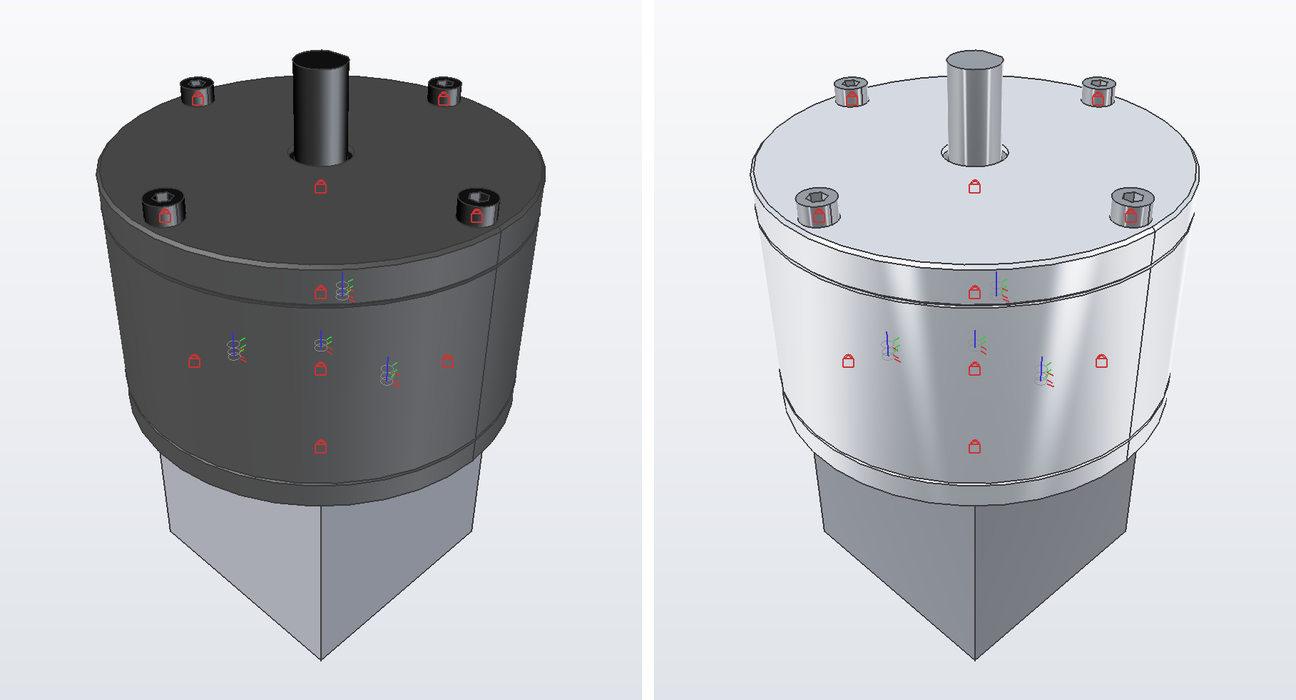
\includegraphics[width=0.9\linewidth]{fig/uix08_gearbox.png}
\caption{The gearbox, FreeCAD's shading (left) and studio shading (right). Same file, same view.}
\label{fig:uix08-gearbox}
\end{figure}

\begin{figure}[!htbp]
\centering
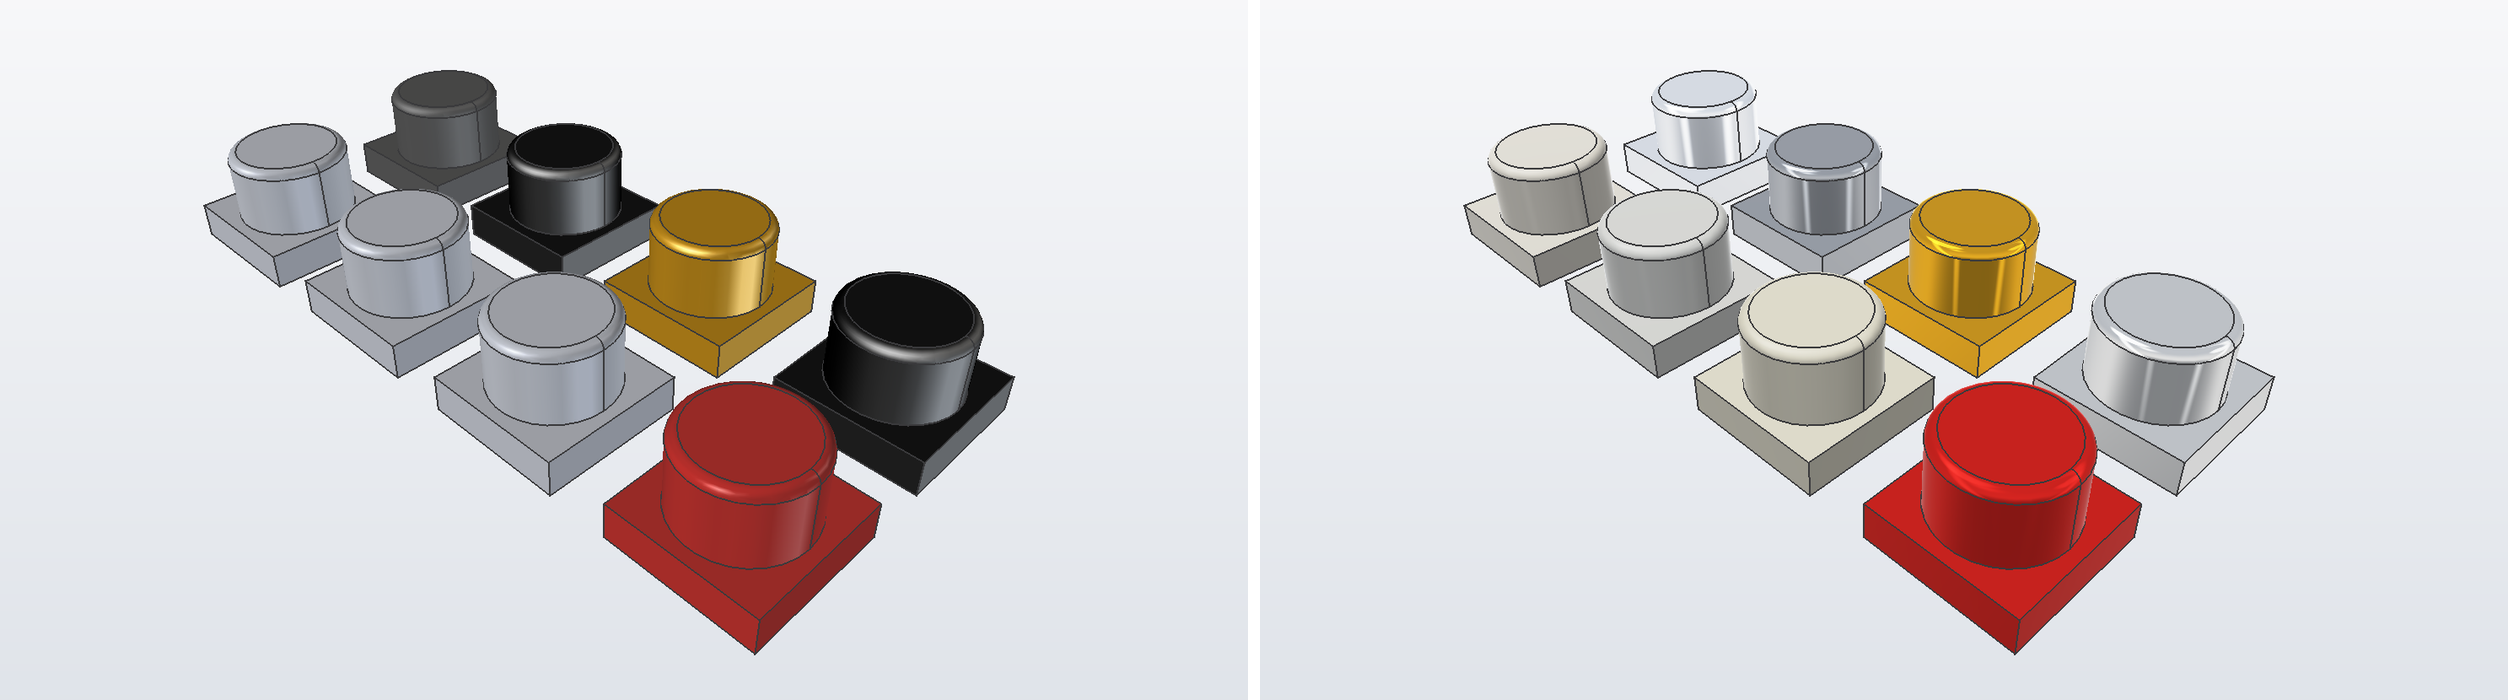
\includegraphics[width=\linewidth]{fig/uix08_materials.png}
\caption{One part per material, FreeCAD (left) and studio (right). Back row, left to right: aluminium 6061-T6,
steel C45, brass, austenitic stainless; front row: ABS, PET, PA6 nylon, and the aluminium coloured red by hand.
FreeCAD shows steel and stainless black and the plastics in its default grey (their cards have no appearance);
the studio gives each its finish, keeps the brass card's own colour and keeps the hand colour.}
\label{fig:uix08-materials}
\end{figure}

%----------------------------------------------------------------------
\subsubsection*{1. How it works}

\begin{itemize}
  \item \textbf{A small shader on the faces only.} \file{bruceworx\_studio.py} puts a GLSL program (Coin's
        \code{SoShaderProgram}) as the first child of the \code{FlatRoot} separator of every Part view provider: the
        faces of Part, PartDesign and assembly parts (a link shares its part's nodes). Edges, vertices, sketches,
        text, draggers and the section caps keep FreeCAD's own drawing, so nothing else can change. Python only,
        no C++.
  \item \textbf{The studio.} A white cyclorama that turns with the camera: a light floor, a bright band just below
        the horizon (which the walls of a part seen from above reflect), a softer sky, three softboxes and two tall
        strip lights that put the bright bands down a turned part. Faces reflect it with a Fresnel term (more at
        grazing angles), blurred by the finish's roughness; a soft key light near the eye and a cool fill; a soft
        shoulder keeps highlights from clipping.
  \item \textbf{The finish from the material} (\code{look\_for}). The card's name, its ``Father'' and its library
        folder pick a look: aluminium, steel, stainless, titanium, brass, bronze, copper, gold, chrome, zinc;
        PETG, ABS, PLA, nylon, POM, PEEK, PTFE, PP/PE, PC/acrylic, PVC, rubber, wood, other plastics. Each has a
        colour, a metalness and a roughness. Rules: FreeCAD's dark metal appearances take the studio's colour; a
        card with its own colour keeps it (a shop card ``PETG Orange'' says what it looks like, and so do the
        BruceWorx electronics cards); \textbf{a colour you set by hand is kept}, with the material's finish (a
        metal then reads as a coating, half metal). A part with no material keeps FreeCAD's colour, satin.
  \item \textbf{Nothing is written to the file.} The look is worked out from the material and the appearance
        whenever either changes (document observers), so a file opens unchanged and shows stock in a stock FreeCAD.
  \item \textbf{What still works as before.} Preselection and selection colours (FreeCAD adds them as emission,
        which the shader keeps), per-face colours and link colour overrides (the material colour is replaced only
        where FreeCAD sends exactly that colour), transparency, \emph{No shading} (Coin's light model reaches the
        shader), textures, clip planes and section views (\code{gl\_ClipVertex}), and the edges sit on the faces as
        before (\code{ftransform}).
  \item \textbf{The vault's iso pictures} (\file{bruceworx\_preview.py}) render the same nodes off screen, so they
        get the studio look for free (Figure~\ref{fig:uix08-iso}); with studio off they are as before.
\end{itemize}

\paragraph{Off switch (\eref{FND-07}).} \emph{Preferences $>$ BruceWorx $>$ Studio shading}, the same switch as
\emph{BruceWorx $>$ Studio Shading} in the menu. Off removes every program node: the scene graph is exactly stock
FreeCAD again (a test checks the face nodes before and after). Like the ground grid, studio shading is drawn only
while the BruceWorx preference pack is applied.

\begin{figure}[!htbp]
\centering
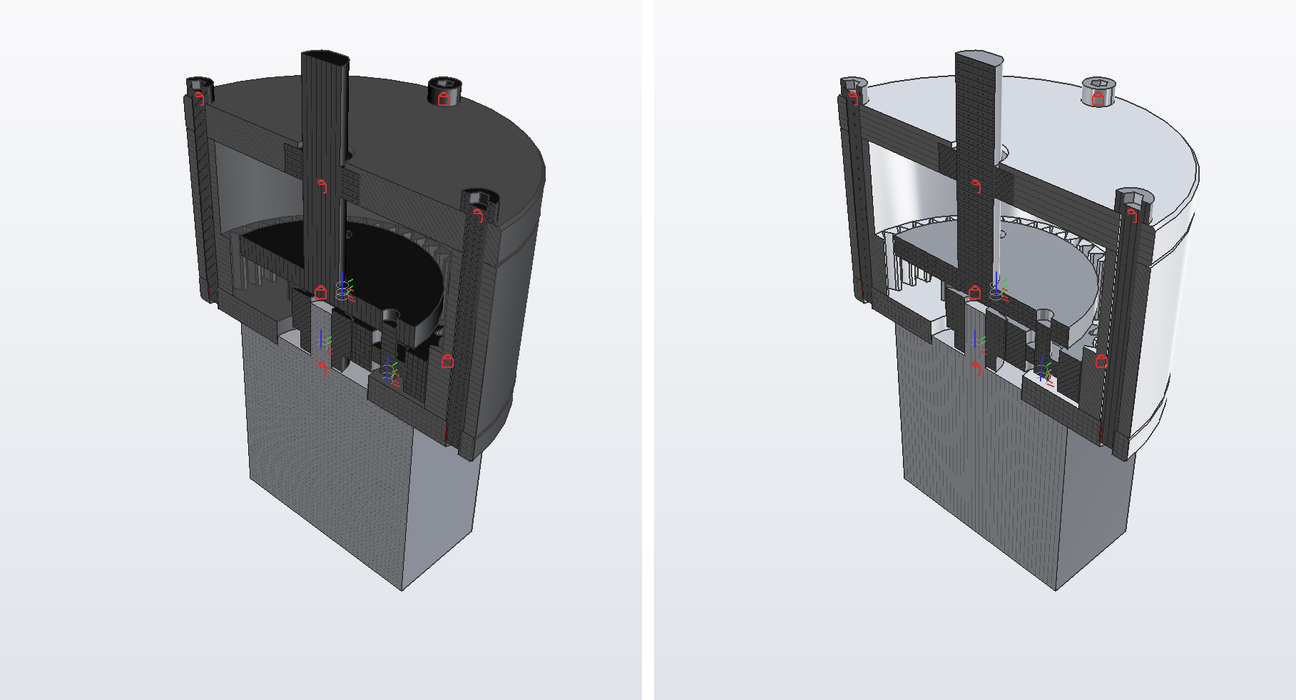
\includegraphics[width=0.9\linewidth]{fig/uix08_section.png}
\caption{Section view (\eref{MOD-16}) with FreeCAD's shading (left) and studio (right). The caps are still drawn by
the section code in the part's FreeCAD colour (dark for aluminium): see question~3.}
\label{fig:uix08-section}
\end{figure}

\begin{figure}[!htbp]
\centering
\begin{minipage}[t]{0.42\linewidth}\centering
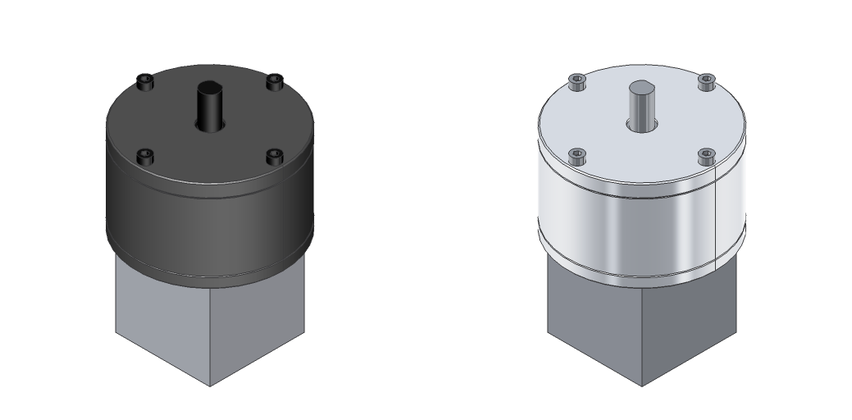
\includegraphics[width=\linewidth]{fig/uix08_iso.png}
\caption{The vault's iso picture of the gearbox, before and after.}
\label{fig:uix08-iso}
\end{minipage}\hfill
\begin{minipage}[t]{0.54\linewidth}\centering
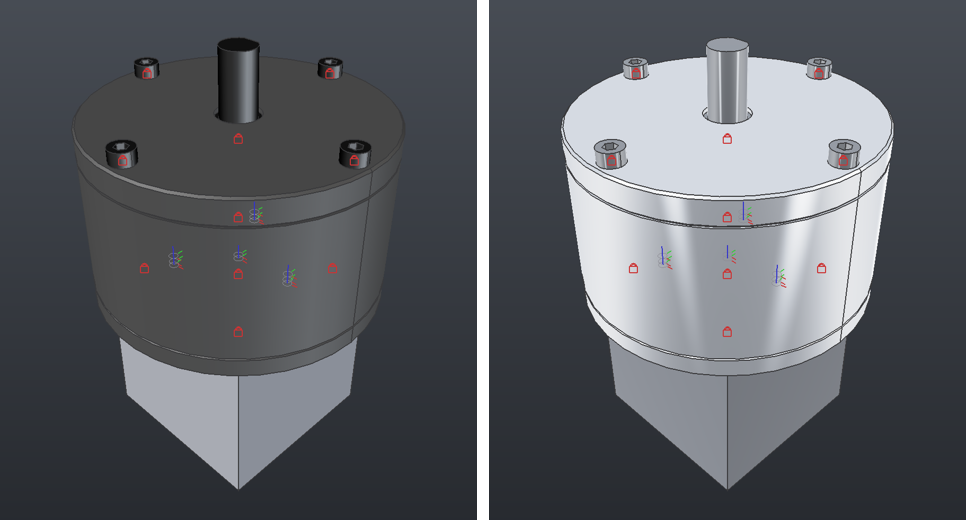
\includegraphics[width=\linewidth]{fig/uix08_dark.png}
\caption{BruceWorx Dark, before and after.}
\label{fig:uix08-dark}
\end{minipage}
\end{figure}

%----------------------------------------------------------------------
\subsubsection*{2. Speed}

Measured on the gearbox (49 parts, a 2056$\times$1942 view, this Mac):
\begin{center}
\small
\begin{tabular}{@{}lrr@{}}
\toprule
 & FreeCAD shading & Studio\\
\midrule
Spinning in the view (frames per second, timer-limited) & 92--97 & 95--99\\
Draw time per frame (FreeCAD's counter) & 1.4--2.0\,ms & 1.6--2.3\,ms\\
Off-screen frame, 1920$\times$1200, with read-back (median) & 48.6\,ms & 49.1--51.2\,ms\\
Bringing the looks up to date (all 49 parts) & --- & 6.9\,ms\\
\bottomrule
\end{tabular}
\end{center}
No visible cost. Two traps were found and fixed on the way: a method call on the material that
\code{obj.ShapeMaterial} returns (\code{hasAppearanceModel}, \code{getAppearanceValue}, \code{getPhysicalValue})
writes it back to the object in FreeCAD~1.1, so reading it in a ``material changed'' observer loops (it held the
spin to 8 frames a second until fixed; the studio now reads only attribute getters, tested); and touching a view
provider in the GUI observer while it is being built crashes FreeCAD. \code{partprops.computed\_mass} has the first
trap too (it calls \code{getPhysicalValue}); see question~6.

%----------------------------------------------------------------------
\subsubsection*{3. Recommendations taken}
\begin{center}
\small
\begin{tabularx}{\linewidth}{@{}p{4.2cm}X@{}}
\toprule
Choice & What I did, and why\\
\midrule
Shader, not textures & A procedural studio in the shader: no image files, sharp at any zoom, nothing to load. A
  cube-map from a photographed studio (HDRI) is the upgrade if you want real-photo reflections.\\
Studio turns with the camera & Every view lit the same way, readable from any side, no per-view bookkeeping (several
  views share the scene graph). A world-fixed studio (reflections slide as you orbit, as in Fusion's ground-plane
  environments) is possible later (question~2).\\
Faces only & The program sits in each part's face node, never at the top of the scene, so edges, sketches, text,
  the navigation cube, the grid and the section caps cannot change.\\
Colour from the material, at draw time & No document writes; hand colours win; a plastic card's own colour wins; the
  stock metal appearances are replaced because they only make sense with the old lights.\\
No ground shadow, no ambient occlusion & Neither is cheap in Coin (shadow maps or a second pass); left for later
  (question~4).\\
Matcap kept for later & A matcap is the studio with the reflections baked into a picture; it would add a second,
  more stylised look (question~5).\\
On by default, one switch & Preference and menu item, the same switch; off is stock.\\
\bottomrule
\end{tabularx}
\end{center}

%----------------------------------------------------------------------
\subsubsection*{4. Tests}
\file{TestBruceWorxStudio.py} (14 tests): the looks of FreeCAD's and shop materials, hand colours, reading a
material without writing it back; in a GUI FreeCAD the program on every part, off $=$ stock nodes, a new part and a
new material followed, the picture changing and the selection still showing, the iso picture rendering. The whole
BruceWorx GUI suite (512 tests, with studio on) passes but for the known SheetMetal test (\code{Mod/SheetMetal} is
not in this build), including \code{TestBruceWorxSection} and \code{TestBruceWorxPreview}.

%----------------------------------------------------------------------
\subsubsection*{5. Questions for you}
\begin{enumerate}
  \item \textbf{Colours of your plastics.} With no colour on the card I chose PETG charcoal (gloss), ABS ivory,
        PLA white, nylon natural, POM white. What colours are your printed and moulded parts? The better fix is a
        colour on the shop cards of \eref{PDM-11} (``PETG Galaxy Black''), which the studio already uses.
  \item \textbf{Studio fixed to the camera or to the world?} Fixed to the camera now (every view lit alike). Fixed to
        the world, reflections slide across the parts as you orbit, closer to Fusion, but a part seen from below
        reflects the floor.
  \item \textbf{Section caps in the studio colour?} The caps come from the section code in the part's FreeCAD colour,
        so an aluminium part is silver with dark grey caps (Figure~\ref{fig:uix08-section}). Shall the caps take the
        studio colour (a small change in \file{bruceworx\_section.py})?
  \item \textbf{A soft shadow under the model} (Fusion's ground shadow), at some cost in speed: wanted?
  \item \textbf{A matcap as a second look} (more stylised, like Onshape or Blender's workbench): wanted, or is one
        studio look enough?
  \item \textbf{FreeCAD writes the material back when it is read through a method} (above). \code{partprops} reads the
        density that way, which touches the body each time the mass is computed. Fix it there (read
        \code{PhysicalProperties} instead)?
  \item \textbf{Brighter or darker aluminium?} The housing reads as polished-bright silver; brushed aluminium in
        Fusion is a little greyer. One number (\code{LOOKS} in \file{bruceworx\_studio.py}) if you want it toned down.
\end{enumerate}
